\documentclass[a4paper,9pt]{scrartcl}
\usepackage{amssymb, amsmath} % needed for math
\usepackage[margin=2.5cm]{geometry} %layout
\usepackage[hyperfootnotes=false, pdfborder={0 0 0}, colorlinks=false]{hyperref}
\usepackage{color}
\usepackage{framed}
\usepackage{enumerate}
\usepackage{csquotes} 
\usepackage{listings}
\usepackage{color}
\usepackage{graphicx}
\usepackage{float}  % For [H] positioning
\usepackage{graphicx}  % For \includegraphics
\usepackage{subcaption}  % If using subfigures

\definecolor{dkgreen}{rgb}{0,0.6,0}
\definecolor{gray}{rgb}{0.5,0.5,0.5}
\definecolor{mauve}{rgb}{0.58,0,0.82}


\setlength{\parskip}{0.4em}
\setlength{\parindent}{3em} 

\makeatletter
\renewcommand{\subsection}{\@startsection{subsection}{2}{0mm}
  {0.25\baselineskip} 
  {0.25\baselineskip} 
  {\normalfont\normalsize\bfseries}}
\makeatother

\makeatletter
\renewcommand{\section}{\@startsection{section}{1}{0mm}
  {1.5\baselineskip}
  {1\baselineskip} 
  {\normalfont\Large\bfseries}}
\makeatother






\newcommand\titletext{"Reinforcement Learning Assignment: FrozenLake"\\ 
\textit{Agents, Multi-Agent Systems and Reinforcement Learning} \\[0.5em] 
\textit{MSc, Artificial Intelligence, 2025}}
\title{\titletext}
\author{Michael Rice}
\usepackage{microtype}

\begin{document}

\maketitle
\section{Introduction}
This report will discuss the results from the second assignment of the CT5134 module. This assignment tackles Reinforcement Learning (RL) via the 
Q-Learning algorithm in the Frozen Lake toy problem, part of the famous 'Grid World' category of problems. Each of the results below are averaged
over a 10 run window. 


\section{Hyperparameter Set 1 - Alpha(0.5), Gamma(0.9), Epsilon(0.1)}

The first set of hyperparameters to test were provided in the assignment and are as stated above. This test can be viewed as being designed to be 
a baseline from which to compare performance to later in the assignment. Below are three figures, each representing a different metric of the 
system's performance/learning. 

Firstly, the leftmost graph below represents the algorithm's reward earned per episode. This can be helpful in understanding the algorithms iterative
improvements over the episodes. As is evident here, the system approaches convergence relatively quickly, then proceeds to oscillate around
the level of convergence for the rest of the episodes. 

Secondly, the plot in the center shows the epsilon value over the length of the experiment. This value is kept constant here but will be varied,
and therefore rendering this plot more relevant, further into these experiments. 

Finally, the rightmost graph depicts the percentage of episodes, averaged again, that reach the 'Win' state. Again, as in the first graph, this
plot shows early convergence followed by stagnation, reaching a peak win rate of just over \textbf{91\%}.

\begin{figure}[H]
\centering
\begin{subfigure}[b]{0.32\textwidth}
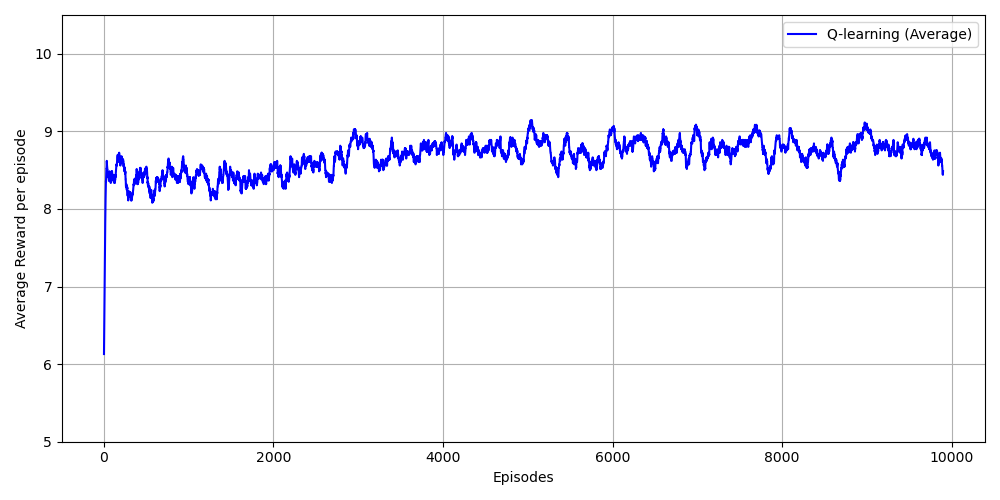
\includegraphics[width=\textwidth]{images/q_learning_rewards_avg(1).png}
\caption{Run Averaged Reward Per Episode}
\label{fig:rewards_avg}
\end{subfigure}
\hfill
\begin{subfigure}[b]{0.32\textwidth}
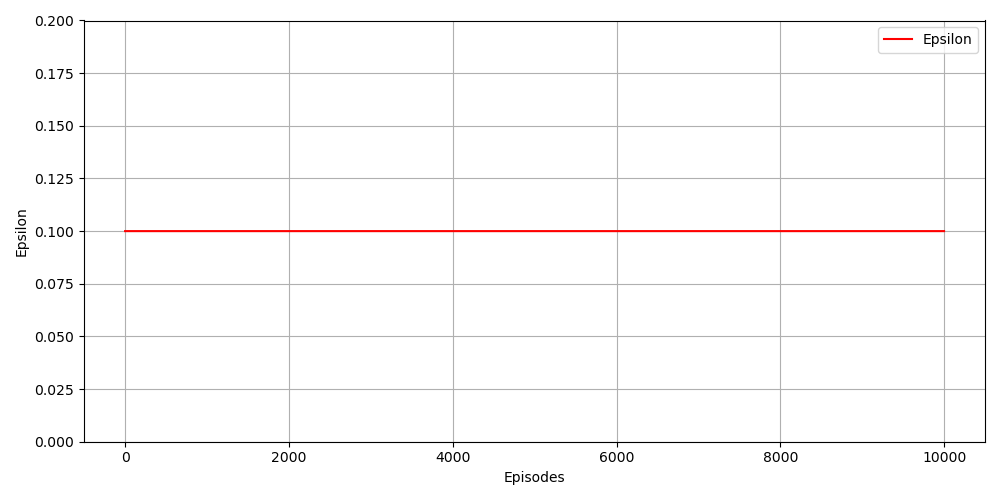
\includegraphics[width=\textwidth]{images/q_learning_epsilon_avg(1).png}
\caption{Run Averaged Epsilon}
\label{fig:epsilon_avg}
\end{subfigure}
\hfill
\begin{subfigure}[b]{0.32\textwidth}
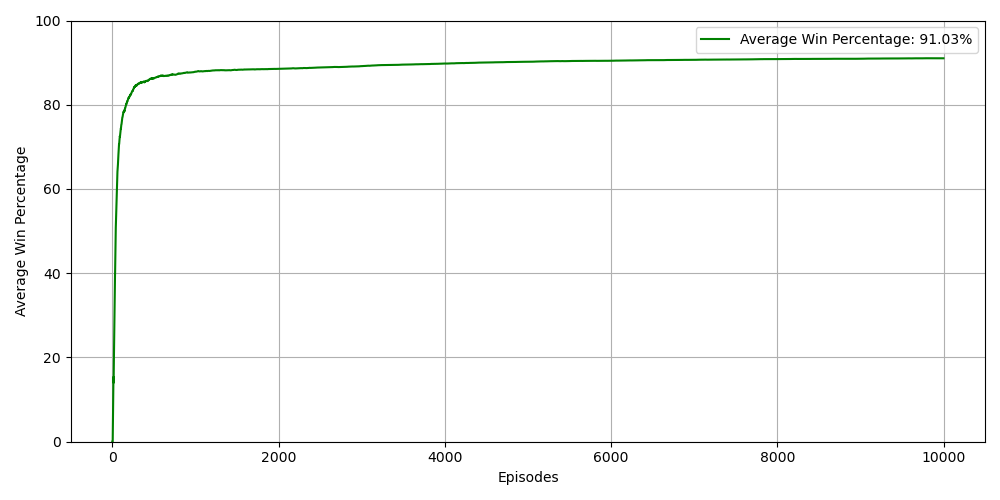
\includegraphics[width=\textwidth]{images/q_learning_win_percentage_avg(1).png}
\caption{Run Averaged Win \% over Episodes}
\label{fig:win_percent_avg}
\end{subfigure}
\caption{Metrics for Hyperparameter Set 1}
\label{fig:training_metrics}
\end{figure}


\begin{figure}[h]
\centering
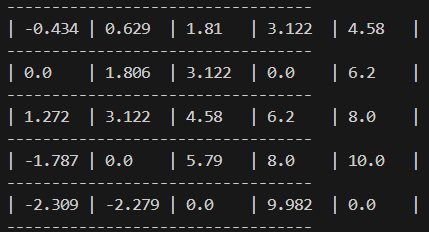
\includegraphics[width=0.5\textwidth]{/home/athen/files/LaTeXStuff/assignments/RL_Assignment2_Report/images/qvalues(1).png}
\caption{Action Value Estimates for Each State}
\label{fig:style_transfer_example}
\end{figure}


\section{Same Hyperparameter Set w/ Epsilon Decay - Linear, Quadratic and Cubic}

In this portion of the experiment, the starting hyperparameters remained the exact same as the section previous. However, this time
throughout each run, the epsilon value would be decayed in order to alter the exploration/exploitation balance to aid in the discovery of
an optimal path through the grid.

Three different methods of epsilon decay were tried during this section of the experiment; Linear, Quadratic and Cubic, each starting at a 
value of 0.1 as before, and ending each run at 0. As can be seen in the plots below, the Linear method retains a constant level of decay
throughout each run, while both the Quadratic and Cubic methods keep larger values of epsilon for longer. This means both of these 
non-linear methods are more explorative at the beginning of the runs, with a faster decay at the end (exploitation).



\begin{figure}[H]
\centering
\begin{subfigure}[b]{0.32\textwidth}
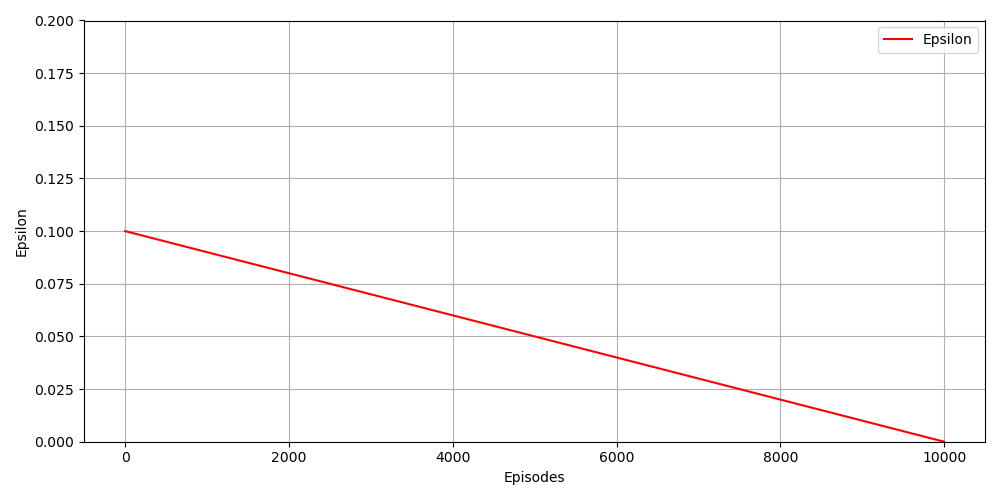
\includegraphics[width=\textwidth]{images/q_learning_epsilon_avg(2)(0).png}
\caption{Run Averaged Epsilon Decay (Linear)}
\label{fig:rewards_avg}
\end{subfigure}
\hfill
\begin{subfigure}[b]{0.32\textwidth}
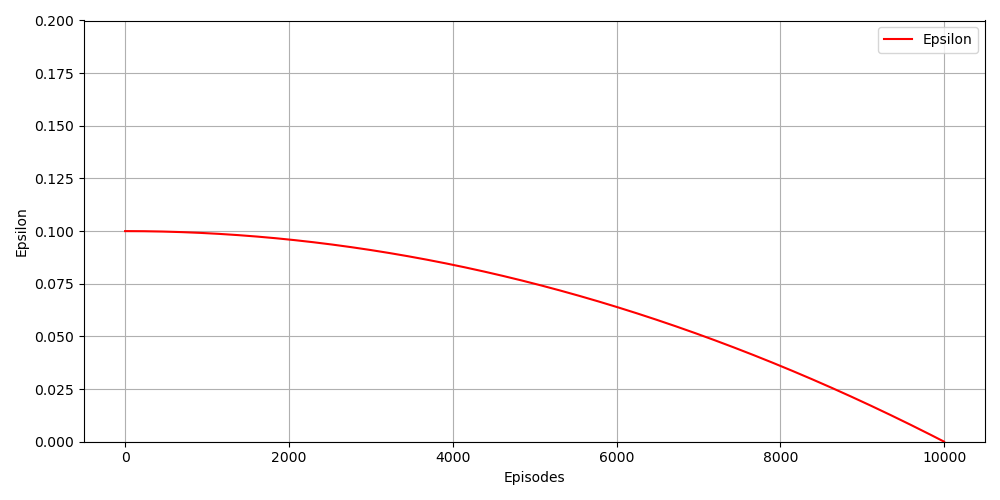
\includegraphics[width=\textwidth]{images/q_learning_epsilon_avg(2)(1).png}
\caption{Run Averaged Epsilon Decay (Quadratic)}
\label{fig:epsilon_avg}
\end{subfigure}
\hfill
\begin{subfigure}[b]{0.32\textwidth}
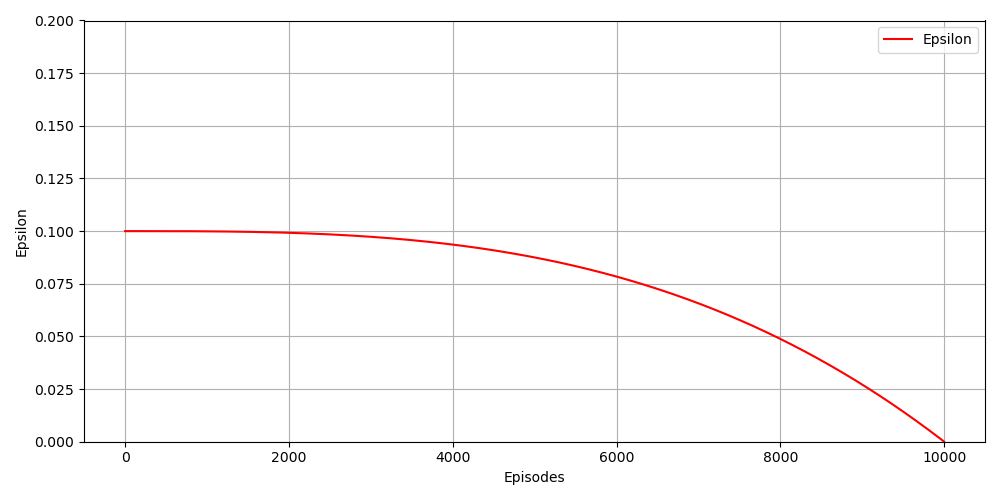
\includegraphics[width=\textwidth]{images/q_learning_epsilon_avg(2)(2).png}
\caption{Run Averaged Epsilon Decay (Cubic)}
\label{fig:win_percent_avg}
\end{subfigure}
\caption{Metrics for Hyperparameter Set 1 w/ Epsilon Decay}
\label{fig:training_metrics}
\end{figure}



\begin{figure}[H]
\centering
\begin{subfigure}[b]{0.45\textwidth}
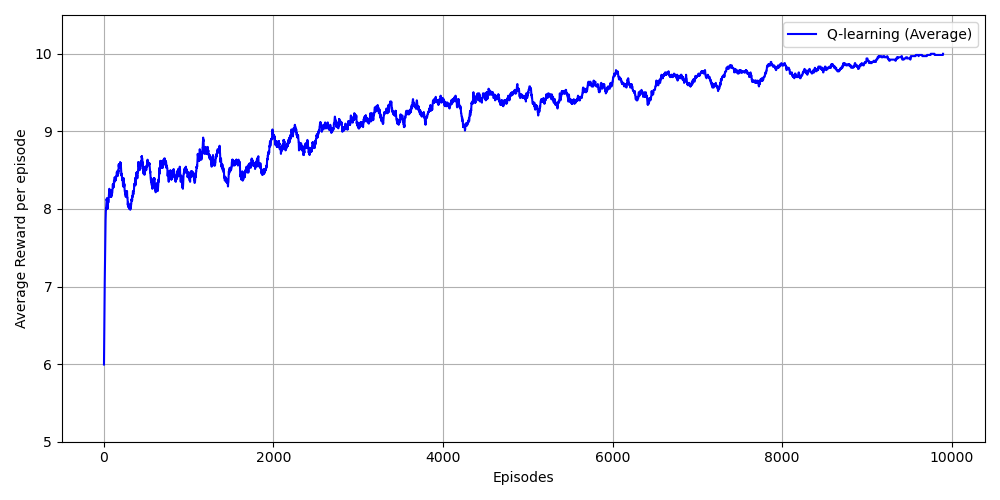
\includegraphics[width=\textwidth]{images/q_learning_rewards_avg(2)(0).png}
\caption{Run Averaged Reward Per Episode}
\label{fig:rewards_avg}
\end{subfigure}
\hfill
\begin{subfigure}[b]{0.45\textwidth}
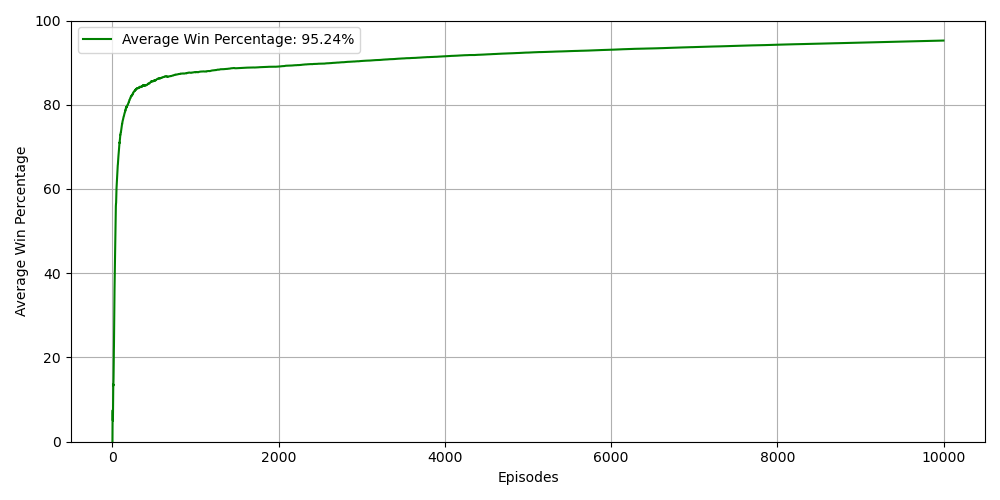
\includegraphics[width=\textwidth]{images/q_learning_win_percentage_avg(2)(0).png}
\caption{Run Averaged Win \% over Episodes}
\label{fig:win_percent_avg}
\end{subfigure}
\caption{Metrics for Hyperparameter Set 1 w/ Epsilon Decay (Quadratic)}
\label{fig:training_metrics}
\end{figure}


\begin{figure}[H]
\centering
\begin{subfigure}[b]{0.32\textwidth}
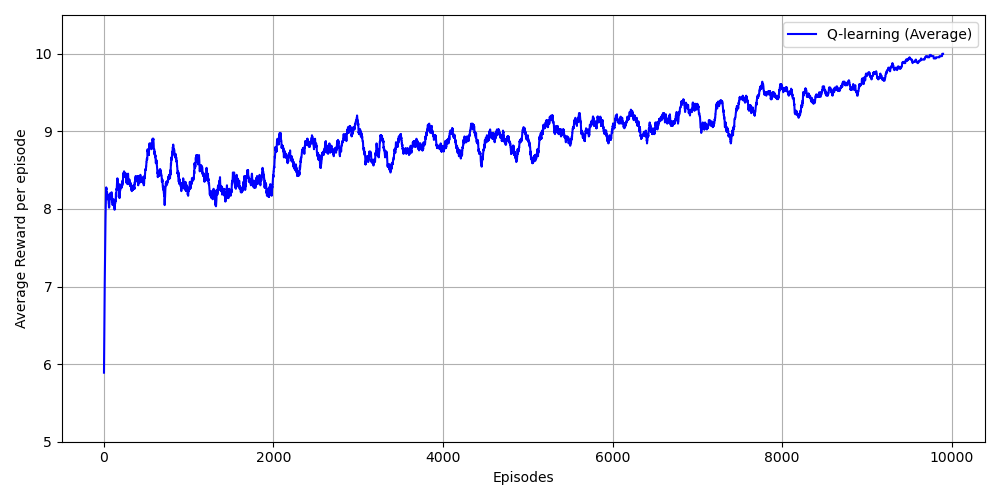
\includegraphics[width=\textwidth]{images/q_learning_rewards_avg(2)(2).png}
\caption{Run Averaged Reward Per Episode}
\label{fig:rewards_avg}
\end{subfigure}
\hfill
\begin{subfigure}[b]{0.32\textwidth}
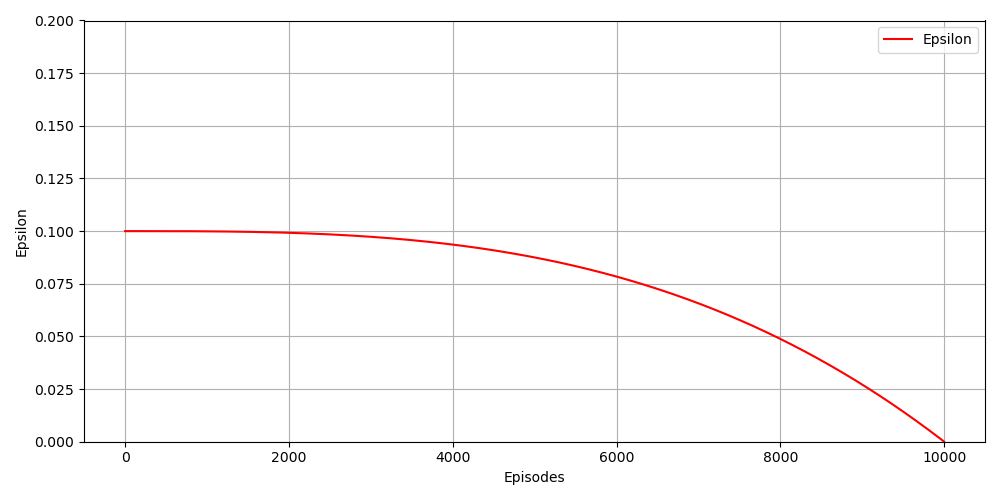
\includegraphics[width=\textwidth]{images/q_learning_epsilon_avg(2)(2).png}
\caption{Run Averaged Epsilon Decay}
\label{fig:epsilon_avg}
\end{subfigure}
\hfill
\begin{subfigure}[b]{0.32\textwidth}
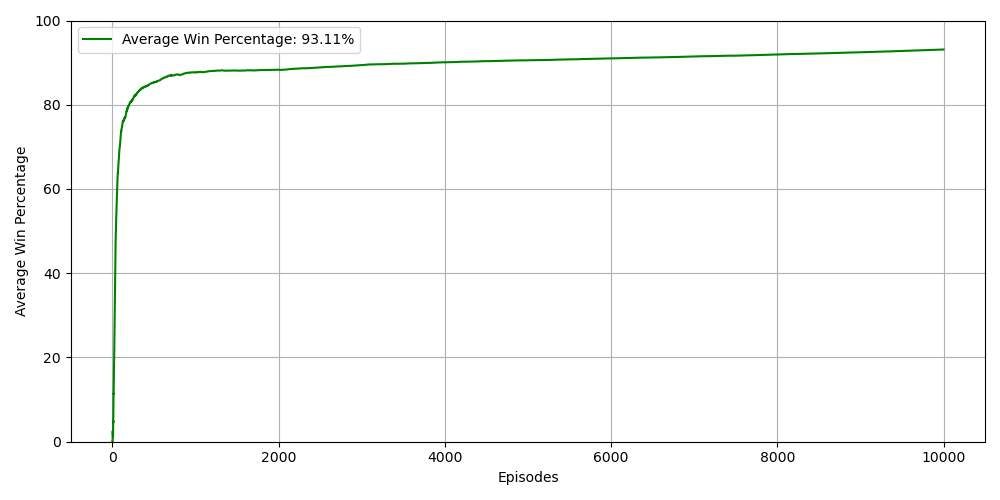
\includegraphics[width=\textwidth]{images/q_learning_win_percentage_avg(2)(2).png}
\caption{Run Averaged Win \% over Episodes}
\label{fig:win_percent_avg}
\end{subfigure}
\caption{Metrics for Hyperparameter Set 1 w/ Epsilon Decay (Cubic)}
\label{fig:training_metrics}
\end{figure}


\section{Hyperparameter Set 3, My Own Choices - Alpha(0.7), Gamma(0.95), Epsilon(0.0)}

Finally, in this section the hyperparameters used were of my own design.




\begin{figure}[H]
\centering
\begin{subfigure}[b]{0.32\textwidth}
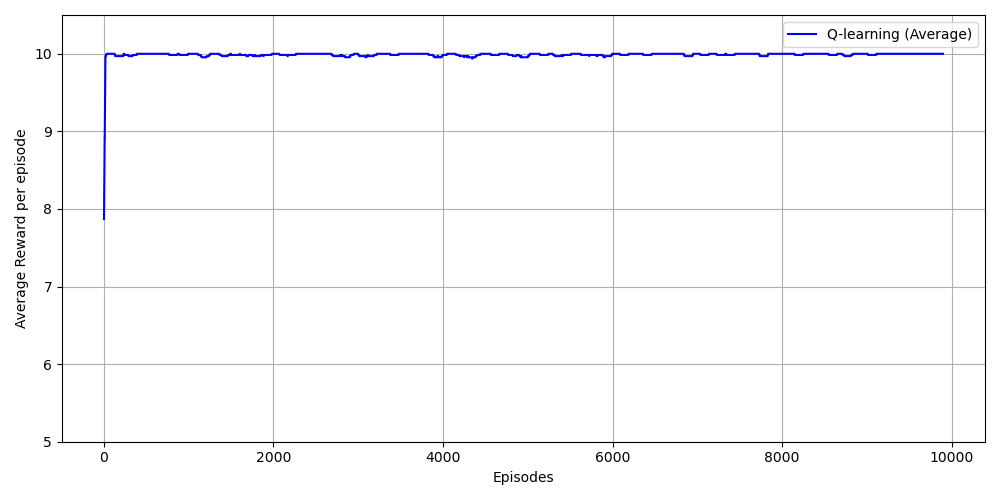
\includegraphics[width=\textwidth]{images/q_learning_rewards_avg(3).png}
\caption{Run Averaged Reward Per Episode}
\label{fig:rewards_avg}
\end{subfigure}
\hfill
\begin{subfigure}[b]{0.32\textwidth}
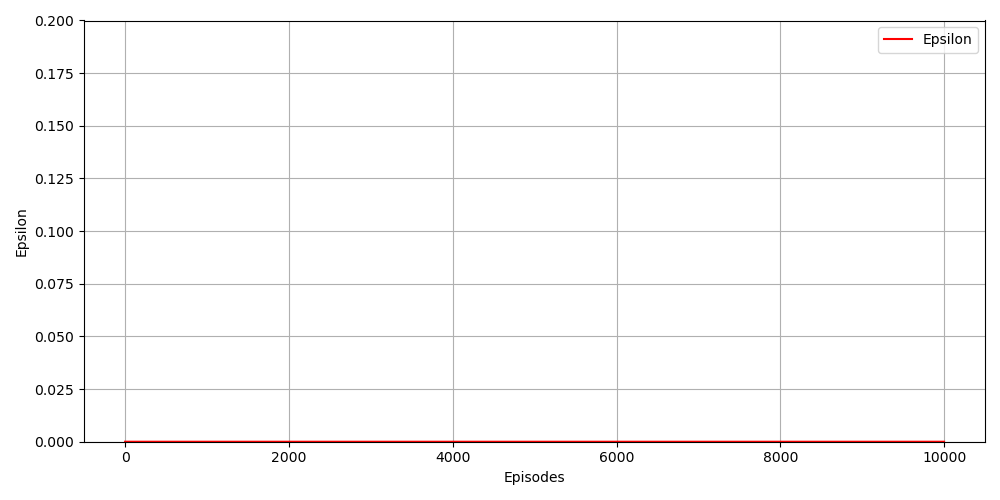
\includegraphics[width=\textwidth]{images/q_learning_epsilon_avg(3).png}
\caption{Run Averaged Epsilon Decay}
\label{fig:epsilon_avg}
\end{subfigure}
\hfill
\begin{subfigure}[b]{0.32\textwidth}
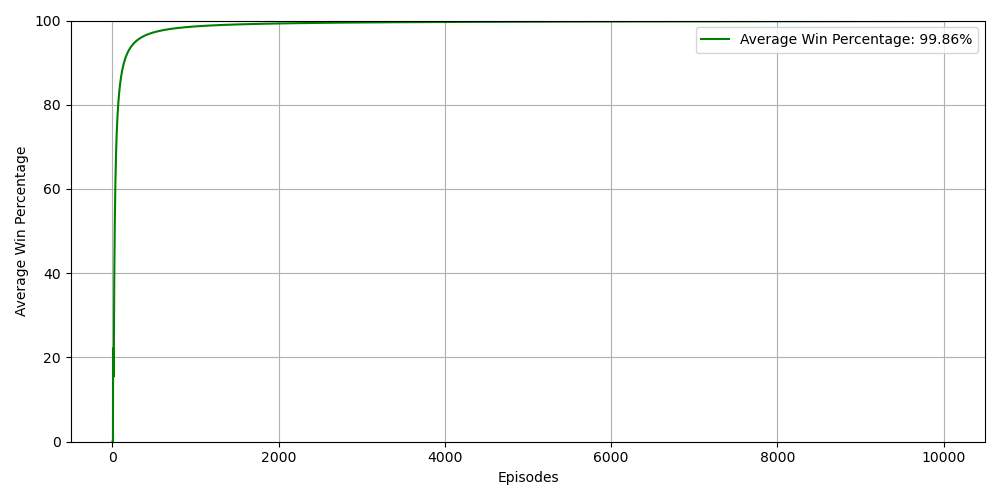
\includegraphics[width=\textwidth]{images/q_learning_win_percentage_avg(3).png}
\caption{Run Averaged Win \% over Episodes}
\label{fig:win_percent_avg}
\end{subfigure}
\caption{Metrics for Hyperparameter Set 3}
\label{fig:training_metrics}
\end{figure}

\begin{figure}[h]
\centering
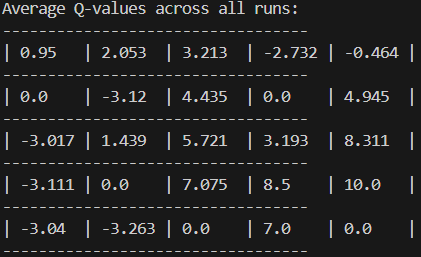
\includegraphics[width=0.5\textwidth]{/home/athen/files/LaTeXStuff/assignments/RL_Assignment2_Report/images/qvalues(3).png}
\caption{Action Value Estimates for Each State}
\label{fig:style_transfer_example}
\end{figure}


\rule{\linewidth}{0.2mm}
% \bibliographystyle{plain}
% \bibliography{/mnt/c/Users/athen/Desktop/MAI_Sem2/AdvancedNLP/Project/NLP_Report.bib}

\end{document}

